% Template for ICASSP-2015 paper; to be used with:
%          spconf.sty  - ICASSP/ICIP LaTeX style file, and
%          IEEEbib.bst - IEEE bibliography style file.
% --------------------------------------------------------------------------
\documentclass{article}
\usepackage{spconf,amsmath,graphicx,qtree,tabularx}
\usepackage{times}
\usepackage{latexsym}
\usepackage{graphicx}
\usepackage{listings}

\usepackage{tikz}
\usetikzlibrary{positioning}
%% Example definitions.
% --------------------
\def\x{{\mathbf x}}
\def\L{{\cal L}}

% Title.
% ------
\title{AUDIO RENDERING OF MATHEMATICAL EQUATIONS}
%
% Single address.
% ---------------
\name{Venkatesh Potluri, Saikrishna Rallabandi, Kishore Prahallad}
\address{Author Affiliation(s)}
%
% For example:
% ------------
%\address{School\\
%	Department\\
%	Address}
%
% Two addresses (uncomment and modify for two-address case).
% ----------------------------------------------------------
%\twoauthors
%  {A. Author-one, B. Author-two\sthanks{Thanks to XYZ agency for funding.}}
%	{School A-B\\
%	Department A-B\\
%	Address A-B}
%  {C. Author-three, D. Author-four\sthanks{The fourth author performed the work
%	while at ...}}
%	{School C-D\\
%	Department C-D\\
%	Address C-D}
%
\begin{document}
%\ninept
\maketitle

\begin{abstract}

Text to speech (TTS) systems hold promise as an information access tool for literate and illiterate including visually challenged. Current TTS systems can convert a typical text into a  natural sounding speech. However, auditory rendering of mathematical content, specifically equation reading is not a trivial task. Mathematical equations have to be read so that appropriate bracketing such as parentheses, superscripts and subscripts are conveyed to the listener in an accurate way. Earlier works have attempted to use pauses as acoustic cues to indicate some of the semantics associated with the mathematical symbols.
In this paper, we first analyse the acoustic cues which human-beings employ while speaking the mathematical content to (visually challenged) listeners and then propose four techniques which render the observed patterns in a text-to-speech system. The evaluation considered eight aspects such as listening effort, content familiarity, accentuation, intonation, etc. Our objective metrics show that a combination of the proposed techniques could render the mathematical equations using a TTS system as good as that of a human-being. To validate the observations from the evaluation, we performed a comprehension test.

\end{abstract}

\section{Introduction}
\label{sec:intro}

Mathematical equations comprise of different types of visual cues to convey their semantic meaning. Some of these visual cues are superscripts, subscripts, parentheses,etc. 
%\subsection{Significance  }
%\label{ssec:significance}
Despite advances in screen reading and text to speech technologies, the problem of speaking complex math remains majorly unsolved. Speaking the equation just as any other string of text, a line, or a sentence will not suffice to effectively render mathematics in speech. For instance, $e^{x+1}-1$ denotes that the value "e" should be multiplied "x+1" times before subtracting 1 from it. However, when it is rendered in speech like a general string, it is difficult to identify the portion of the equation in the superscript and the remainder of it after the superscript.
To effectively resolve such ambiguities and identify such demarcations in mathematical content, information presented through visual cues such as spatialisation must be mapped to their auditory equivalent. Mathematics, in its visual form, gives the reader a very high level granularity in perceiving the equation. Mathematical equations, when presented in audio must be able to match the advantage in granularity provided in visual representation of mathematics.   The typical issues in audio rendering of mathematical equations include quantification, superscripting and subscripting, and fractions.

%\subsection{Review of the Existing Methods}
%\label{ssec:previous}
\subsection{Quantification}
\label{ssec:quantify}
Most of mathematical equations contain expressions in parentheses. For instance, considering the equation
$(A+B)*(C+D)+E$, it may seem that the equation can just be treated as a general string of text while speaking. However, this will create a confusion in the listener, as there are two ways of expressing.
%The equation could be spoken as 
\begin{itemize}
\item  "left parenthesis A plus B right parenthesis times left parenthesis C plus D right parenthesis plus E " 
\item " A plus B times C plus D plus E ". 
\end{itemize}
In the former case, the listener will have to keep a track of all the parentheses when he or she listens to the equation. This becomes a hectic task for bigger equations and also results in deviating the listener's attention from concentrating on the actual contents of the equation. On the other hand, in the latter case, the listener gets an ambiguous representation of the equation. The spoken form of the equation should have additional information to the equation to solve this ambiguity.
%\Tree[.A [.(B*C)]]

\subsection{Superscript and subscript}
\label{ssec:supsub}
Today's screen readers and TTS engines do not effectively convey the equations with superscript and subscript content. They often do not speak out the parts of the equation contained in the superscript and subscript. They often speak out such content continuously, with the rest of the equation. For instance, let us say the expression is $E^X$. With the currently available technologies, the expression may be rendered as "EX". This does not give the listener the information that X is in the superscript and the listener may understand the expression as $E*X$. In expressions where there are at least 2 variables that cause a phonetic sound when spoken together, the general TTS may treat the expression as a complete word. consider the expression $A^B$. The TTS may speak it as "ab"Äù. In case of numbers, say we have an expression $5^{2^5}$, the TTS reads it as "five hundred twenty five"Äù or "Äúfive two five"Äù. We come across the same issues while trying to render subscript text. If a human speaks the expression, he may not make such mistakes. The challenge to the human speaker lies in effectively conveying the spatial orientation of the different parts of the equation. That is, the equation, presented in audio must give the listener a clear picture of what content is in the superscript and the subscript. The listener must also be able to observe the end of the super script or subscript part of a mathematical expression. The listener should understand that any thing that he listens to after the end is in the baseline or the general part of the equation, unless specified. To overcome this challenge, the spoken form of an equation should  provide the listener with different cues for superscript and subscript content.

\subsection{Fractions}
\label{ssec:fractions}
Fractions, like the other mathematical concepts discussed above can not be treated like a general string of text. The key information that has to be conveyed to the listener in addition to the contents of the fraction is the beginning of the fraction, the content of the fraction in numerator and denominator and the end of the fraction. The audio equivalent of the equation should effectively be able to convey nested fractions in addition to the regular fractions to the listener. \\


There have been several attempts to present mathematical content through alternative modes to vision. Efforts have been made to formulate standards for presenting math through Braille and speech. Nemeth Code\cite{nemeth1973nemeth} is a special type of Braille used for math and science notations. With Nemeth Code, one can render all mathematical and technical documents into six-dot Braille. This code could also be used to speak mathematical content.
Dr T.V Raman has developed an audio system for technical readings (ASTER)\cite{raman1998audio}. ASTER is a computing system for producing audio renderings of electronic documents. The present implementation works with documents written in the TEX family of markup languages: TEX, LaTeX and AMS-TEX. A more recent attempt has been made by a company called design science. They developed an internet explorer plugin called MathPlayer \cite{soiffer2005mathplayer} that displays and speaks out mathematical content marked up in MathML \cite{ion1998mathematical}. There have been attempts to form a set of guidelines to effectively speak mathematics in audio. The handbook for spoken mathematics \cite{chang1983handbook} gives an account of such an attempt. An article on how to speak math \cite{fateman1998can} also describes the challenges in speaking mathematics to and by a computer.

Earlier works discussed so far, have not effectively  used paralinguistic cues and variations in the equation. However, humans use a lot of cues when reading out a mathematical equation which helps in understanding the semantics of it. Usage of the cues similar to the humans would result in more effective rendering of the equations.   

The objective of this paper is to analyse the way these visual cues are presented in an auditory format by human speakers who are well acquainted with speaking the mathematical content especially to visually challenged individuals. A subjective and objective analysis is performed on the equations recorded by the speakers. Based on this analysis, we make an attempt to form specific rules to map the visual cues to their auditory equivalents to programatically and unambiguously render the mathematical content in audio using a text-to-speech system.
%Section \ref{ssec:significance} discusses the importance of the problem at hand and Section \ref{ssec:previous} gives an overview of some of the efforts made by other researchers in this regard. 

Section \ref{sec:cues} discusses the  significance of the cues in rendering mathematical equations in audio and the idea behind this study.  Section \ref{sec:techniques} discusses the proposed ideas and provides details on the qualitative analysis of the proposed ideas. Section \ref{sec:comprehension} gives the specifics and the results of the comprehension test.

\section{Cues in spoken equations}
\label{sec:cues}


Our study is based on the preposition that treating a mathematical expression as a regular English sentence while speaking is not an effective way to present mathematical content in an auditory form. In order to test this observation, we asked a set of 15 people to rate mathematical equations spoken by a traditional TTS system.  Then we conducted the same experiment on spoken equations (i.e., equations spoken by a human-being). The details of the listening tests are as follows.




\subsection{Procedure for the listening tests}
\begin{figure}[h]
\label{fig:eval}

\begin{minipage}[b]{1.0\linewidth}
  \centering
  
  \centerline{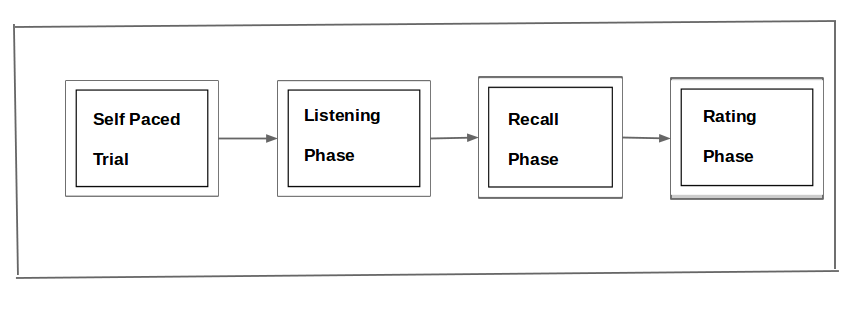
\includegraphics[width=8.5cm]{eval}}
 
%  \vspace{2.0cm}
  \centerline{Fig: Evaluation procedure}\medskip
\end{minipage}
\end{figure}

A set of 15 participants were made to listen to the recorded equations. Each participant was made to listen to the equations using headphones and the responses were recorded. The listening test was self paced and also the users were informed that they were free to listen to the equation any number of times till they felt comfortable that they could recall the equation.  Similarly, the same participants were also made to listen to speech of mathematical equations generated by a TTS system. The participant will have to reproduce the equation he/she listens to. In addition to reproducing the equation, the participant will have to evaluate the spoken equation based on eight other parameters, i.e., perform objective analysis. We arrived at these parameters partly by following the listening test procedures followed in the Blizzard challenges \cite{hinterleitner2011evaluation} and our own analysis.



\subsection{Selection of the equations}
\label{ssec:equations}

Selection  of suitable equations is a critical component to analyse the auditory presentation of mathematical content. We hand picked a few equations which had variations in number of variables, number of sub expressions and length of the equation. Each of the equations is semantically unrelated, that is, the equations have mathematical content but the listener may not have come across the exact same equation prior to listening to them from our recordings . The reason behind choosing the equations in such a way is to ensure that the listener's prior knowledge does not influence the ability to recall the equation. If the listener is able to recall the equation even before he or she listens to it completely, the listener is benefitting from memory, not the spoken equation.


\begin{table}[t]
\caption{\label{tts}Evaluation of Spoken Math vs TTS}

\vspace{8pt} % Gap between title and text

% title of Table
\centering
\begin{tabular}{|l |c |c|}
% centered columns (4 columns)
\hline%\hline %inserts double horizontal lines
Parameter & Spoken & Synthesized  \\
                  &              & (Technique 1) \\[0.5ex]
% inserts table
%heading
\hline
% inserts single horizontal line

Listening Effort & 2.5 & 4.4 \\
\hline
Content Familiarity &2.7 &2.7 \\
\hline
Effectiveness of & & \\
additional cues &3.2 &1.2 \\
\hline
Accentuation &4.3 &2.5 \\
\hline
Intonation & 4.26 & 1.6  \\
\hline
% inserting body of the table
%Pitch  Variation& 4.17 & 1.4 \\
%\hline
Pauses & 3.1 & 2.15 \\
\hline
Number of repetitions & & \\
(Mode) &2 & 4 \\
\hline
Mean Opinion Score & 4.42 & 1.89  \\%[1ex]
\hline
% [1ex] adds vertical space

%inserts single line


\end{tabular}
\end{table}


\subsection{Parameters for objective analysis}
\label{ssec:parameters}

On a scale of 1 to 5, the participants were asked to evaluate the spoken equations on the following parameters.
\begin{itemize} 
 \item Listening effort (1 = low, 5 = high)
 \item Intonation (1 = ineffective and 5 = very effective)
 \item Acceptance (1 = poor, 5 = good).
 \item Speech pauses ( 1= not noticeable and 5 = very prominent)
 \item Accentuation (1 = poor and 5 = very prominent).
 \item Content familiarity (1 = totally new concept and 5 = very familiar).
 Here 1 indicates that the user is not acquainted to the terminology used in the equation. In this case, the participantÄôs' response for that particular equation can not be considered completely as he may have entered a wrong response due to the lack of domain knowledge, not due to the lack of understanding of the audio.
 \item   Effectiveness of additional cues such as sounds, pitch and rate variations, change in direction, etc. (1 = hardly noticeable and 5 = very helpful).
 \item   Number of repetitions of each equation.
\end{itemize}

\subsection{Inferences from the listening test}
\label{ssec:listening1}
The results of this experiment, shown in the Table ~\ref{tts}   indicate that the equations are not intelligible enough if it is spoken as a plain text using a text-to-speech system. The mean opinion scores of spoken equations indicate a human-being use several acoustic cues to manifest the semantics of the mathematical symbols in audio mode. It was noticed that the trained speakers brought certain variations in their speech while speaking specific aspects of the mathematical expression. The variations are noticed in pauses and pitch variations (intonation). 
A careful analysis revealed that the acoustic variations were introduced by the speakers to unambiguously speak 1) quantification, 2) superscripting and subscripting and 3) handling fractions in mathematical equations. 

%Sections ~\ref{ssec:quantify} to ~\ref{ssec:fractions}  explain the ambiguities that a listener may come across if the mathematical equation is not spoken with care.

Based on the feedback received from participants, we can infer that the use of these additional cues can effectively and unambiguously present mathematical content in audio.   The question is how to introduce such cues to synthesise a mathematical equation using a text-to-speech system.


\section{Proposed techniques}
\label{sec:techniques}
With the advent of languages like MathML, it is possible to programatically identify different attributes and visual cues of a mathematical expression. This possibility can in turn be leveraged to make some modifications  while generating speech for mathematical content.  We propose four techniques that could enhance the way mathematical content is rendered in audio.

\begin{figure}[h]
\label{fig:res}

\begin{minipage}[b]{1.0\linewidth}
  \centering
  
  \centerline{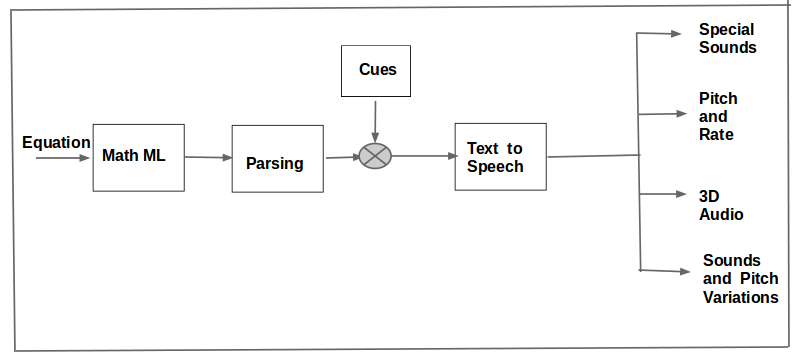
\includegraphics[width=8.5cm]{block}}
 
%  \vspace{2.0cm}
  \centerline{Fig: Overall framework for the proposed techniques}\medskip
\end{minipage}
\end{figure}

An example depicting the workflow of the entire algorithm is shown in the Figure 1. For the sake of illustration, a simple expression , $(X+Y)^{4-2} $ was taken :

\begin{figure}[t]
\caption{Example Synthesis using a simple expression}
\vspace{8pt}
\resizebox{8cm}{12cm}{
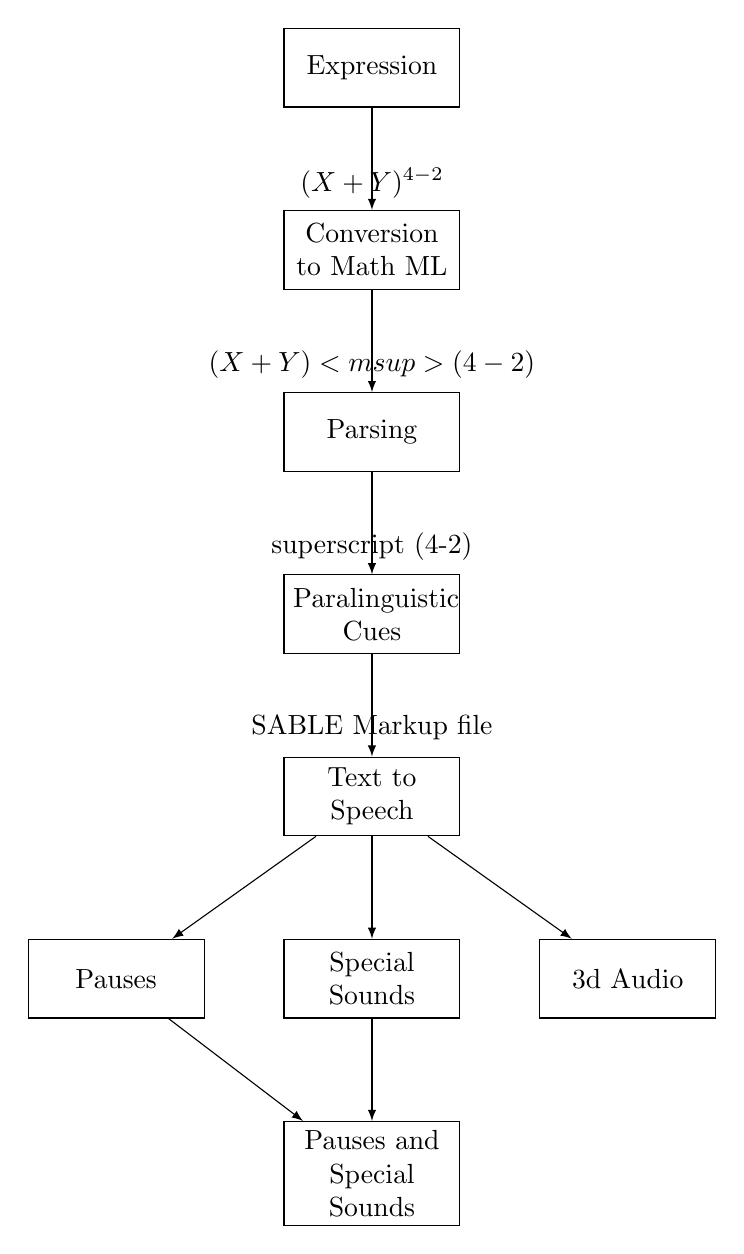
\begin{tikzpicture}[
node distance=1.3cm and 1cm,
ar/.style={->,>=latex},
mynode/.style={
  draw,
  text width=2cm,
  minimum height=1cm,
  align=center
  }
]
\node[mynode] (expression) { Expression};
\node[mynode,below=of expression] (MML) {Conversion to Math ML};
\node[mynode,below=of MML] (Parse) {Parsing};
\node[mynode,below=of Parse] (Cue) {Paralinguistic Cues};
\node[mynode,below =of Cue] (TTS) {Text to Speech};
\node[mynode,below left=of TTS] (1) { Pauses};
\node[mynode,below=of TTS] (2) {Special Sounds};
\node[mynode,below right=of TTS] (3) { 3d Audio};
\node[mynode,below right =of 1] (4) {Pauses and Special Sounds};

\draw[ar] 
  (expression) -- node[below] {$(X+Y)^{4-2} $} (MML);

\draw[ar] 
  (MML) -- node[below] { $(X+Y) <msup> {(4-2)}$} (Parse);

\draw[ar] 
  (Parse) -- node[below] {superscript (4-2)} (Cue);

\draw[ar] 
  (Cue) -- node[below] {SABLE Markup file} (TTS);

\draw[ar] 
  (TTS) -- node[below left] {} (1);

\draw[ar] 
  (TTS) -- node[below ] {} (2);

\draw[ar] 
  (TTS) -- node[below right ] {} (3);

\draw[ar] 
  (1) -- node[below  ] {} (4);

\draw[ar] 
  (2) -- node[below  ] {} (4);

\end{tikzpicture}
}
\end{figure}

The Equation was first converted into the Math Markup Language format. We chose "Presentation" Markup style to represent the equations.  
It is then text processed to identify and segregate the different terms occurring in the equation. The following terms have been segregated.

\begin{itemize}
\item Subscripts and superscripts 
\item Fractions
\item Square root terms
\item Overscripts and underscript
\end{itemize}

The MathML representation is processed to convert it into natural language and the acoustic cues such as pauses, intonation are incorporated to generate a file in the SABLE markup language \cite{sproat1998sable}. 
%Here's an example of the SABLE file:
The SABLE file is input to the speech synthesis system which generates the audio form of the equation with specified pauses and intonation. We have generated the audio files using the Festival Speech Synthesis System\cite{black2002festival}. 
Sections 4.1 through 4.4 discuss each of the four proposed techniques. 



\subsection{ Technique 1 : Rendering equations with pauses and special sounds}
\label{ssec:t2}

In visual communication, icons and symbols are used as indications for some types of information. In the context of mathematical expressions, the user can perceive the type of elements ( superscripts, subscripts, etc ) by getting a glance at the equation. A person has the advantage of perceiving a lot of information of the equation even before looking at the actual contents of the equation. This technique attempts to present the equation in a manner that a person gets a similar advantage when he listens to it.\\

 In this concept, we made use of special sounds or ear cons while presenting the equations. However, replacing speech with sounds alone is not the most effective way to tackle the problem of presenting mathematic equations in audio. We made use of paralinguistic cues including, but not limited to sounds.

The cues presented in this method include:
\begin{itemize}
\item \textbf{Pauses} to convey certain parts of an equation.
These pauses are mainly used to separate the parts of mathematical expressions. Consider $(A+B)^2$ and $(A+B^2)+1$.
It would sound more natural and intuitive if the expressions are spoken as ``the quantity A + B pause superscript 2 " and ``the quantity A + B superscript 2 pause + 1 .
\item \textbf{Sounds} to indicate certain symbols and mathematical operations.  Sounds are used to indicate superscripts, subscripts, roots, under scripts, over scripts and under script-over script combination.
\end{itemize}
We chose the sounds(such as the sound ``ding"Äù) such that would be pleasant to the ear and that are passively noticed by a listener so as not to distract too much, at the same time, are loud enough not to go unnoticed. The sounds show a transition from high to low and low to high when there is a subscript and superscript respectively. Any other type of sounds  and their variations could also be applied in this technique.


\begin{table}[t]
\caption{Pitch and rate variations}

\vspace{8pt} % Gap between title and text

% title of Table
\centering
% used for centering table
\begin{tabular}{|l | c | c | }
% centered columns (4 columns)
\hline%\hline %inserts double horizontal lines
Term & Pitch variation & Rate variation \\[0.5ex]
% inserts table
%heading
\hline
% inserts single horizontal line
Superscript & 50 & 20  \\
% inserting body of the table
Subscript & -50 & -20  \\
Fraction & 25 & -25  \\
Underscript & -60 & -25  \\
Overscript & 60 & 25\\ %[1ex]
% [1ex] adds vertical space
\hline
%inserts single line


\end{tabular}
\label{table:pitchandrate}
% is used
%to refer this table in the text
\end{table}



\begin{table*}[t]
\centering
\caption{Evaluation of the proposed techniques}

\vspace{8pt} % Gap between title and text

% title of Table
%\centering
% used for centering table
\begin{tabularx}{\textwidth}{|l |c |c |c |c|}
% centered columns (4 columns)
\hline%\hline %inserts double horizontal lines
Parameter   & Technique\#1 & Technique\#2 & Technique\#3 & Technique\#4 \\[0.5ex]
% inserts table
%heading
\hline
% inserts single horizontal line
Intonation Variation  & 2.3 & \textbf{4.7} & 4.32 & 4.68 \\
\hline
% inserting body of the table
Pitch  Variation & 1.4 & 4.43 & \textbf{4.82} & 4.36\\
\hline
Pauses  & \textbf{4.15} & 3.7 & 3.7 & 3.87 \\
\hline
Listening Effort  & 3.5 & \textbf{2.3} & 2.64 & 2.47\\
\hline
Content Familiarity  &2.7 &2.7 &2.7 &2.7\\
\hline
Effectiveness of additional cues  &1.82 & 4.32 & \textbf{4.37} & 4.23\\
\hline
Accentuation &\textbf{3.47} & 2.3 & 3.2 & 3.6 \\
\hline
Number of repititions(Mode) & 3 & 2 & 2 & 2\\
\hline
Mean Opinion Score  & 2.27 & 4.37 & \textbf{4.62} & 4.35\\ %[1ex]
% [1ex] adds vertical space
\hline
%inserts single line


\end{tabularx}
\label{table:eval}
% is used
%to refer this table in the text
\end{table*}
%\end{center}

  %\centering


\subsection{Technique 2 : Rendering equations with pitch and rate variations}
\label{ssec:t3}

Screen Reader users are familiar to pitch changes. Generally, a high pitch is used to denote capitals and a low pitch is used to denote tool tip messages. On observing the human recorded equations explained in Section \ref{sec:cues}, we observed that speakers tend to modulate the pitch as they read aloud certain parts of a mathematical expression. It has been observed that certain parts of a mathematical expression are spoken at a faster rate to indicate that it is a sub expression and to isolate it from the rest of the expression. \\

In this technique, we use pitch and rate changes to denote the presence of certain mathematical attributes. The pitch and rate increase while speaking out the superscript text and decrease while speaking the subscript text. A similar method can be employed to properly render fractions. The numerator is spoken in a higher pitch and the denominator is spoken in a lower pitch. Similarly, quantities in a root are spoken at a faster rate. Table \ref{table:pitchandrate} shows the pitch and rate variation(in percentage) that are applied to the Mathematical equation. The variation is with respect to the base pitch and rate of the TTS.


\subsection{Technique 3: Rendering equations with audio spatialisation}
\label{ssec:t4}
In this technique, we made an attempt to draw a closer analogy to the spatial positioning of various variables and numbers of a mathematical equation. The listener can be given the illusion that the superscript part of the math expression is spoken from above his head and the rest at the usual level using the Head Related Transfer Function (HRTF) \cite{geronazzo2011head}.
Table 
\ref{table:hrtf} shows the sets of angles chosen for the different parts of the equation such as superscript, etc. 



\begin{table}[h]
\caption{Sets of HRTF angles for audio spatialisation}

\vspace{8pt} % Gap between title and tex

% title of Table
\centering
% used for centering table
\begin{tabular}{| c | c | c |}
% centered columns (4 columns)
\hline%\hline %inserts double horizontal lines
Term & Elevation Angle & Azimuth Angle \\[0.5ex]
% inserts table
%heading
\hline
% inserts single horizontal line
Superscript & 90 & 30  \\
% inserting body of the table
Subscript & -90 & 30  \\
Fraction & 270 & 45  \\
Underscript & -90 & 45  \\
Overscript & 90 & 30\\ %[1ex]
% [1ex] adds vertical space
\hline
%inserts single line


\end{tabular}
\label{table:hrtf}
% is used
%to refer this table in the text
\end{table}


We identify the portions of a mathematical expression that require modification in spatial orientation of sound. Based on the attribute, we apply the HRTF function with the required angles.


\subsection{Technique 4 : Rendering equations with pitch variations and special tones}
\label{ssec:t5}


In this technique, we render the equations in audio by varying the pitch, adding pauses, emphasising the speech and adding sounds at required parts of a mathematical expression. As explained in 3.3, we can make pitch and rate manipulation while rendering superscripts, subscripts, fractions, under scripts and over scripts. In addition to the variations in speech, we have also added sounds to indicate the listener before hand that he must expect one of the above mentioned variations ( superscripts, subscripts, etc). The sounds used here are the same as the ones mentioned in section 3.2.
The Pitch and rate variations that are introduced are the same as the percentage values given in table \ref{table:pitchandrate}.


\subsection{Analysis of the Listening test}
\label{ssec:ideaseval}


A system was built to render mathematical expressions implementing each of the proposed ideas. An experiment procedure similar to the one explained in Section \ref{sec:cues} was followed. 30 participants were made to participate in the experiment. The table contains the normalised scores(1 to 5) calculated over the responses for the equations. The number of repetitions of the equation has the  mode value( most occurring value).

On analysing the experiment as described in Section \ref{sec:cues}, it is observed that the participants are able to understand the human spoken equations. More over, it can be clearly understood that generating spoken forms of mathematical equations without making any enhancements is not capable of rendering math effectively. It can also be inferred that making use of just  a few paralinguistic cues, sounds and pauses as explained in section \ref{ssec:t2} will not suffice either. The pitch and rate changes while rendering certain parts of the mathematical expressions have proven to be helpful to the participants in comprehending the expression. In the method described in section \ref{ssec:t4}, the listener has been able to draw an analogy to the print form of mathematics. It has been observed that the method explained in section \ref{ssec:t2} did not prove to be helpful to the listeners. However, from the table \ref{table:eval} and the values corresponding to the technique explained in section \ref{ssec:t5}, it is evident that use of  cues (pauses and rate variations ) in addition to special sounds can be significantly effective in helping a listener.(see the demonstration of the listening test on the webpage associated to this paper: http://goo.gl/FLTIOv).

\section{Evaluating the Comprehension}
\label{sec:comprehension}

In our previous experiments, we showed that the traditional TTS technology can not convey mathematics unambiguously and evaluated our proposed ideas based on a fixed set of parameters. From this evaluation, we could observe that people were able to get a clearer understanding of the equations with spatially oriented audio(\ref{ssec:t4}). To objectively validate this observation, we performed a comprehension test.  We perform this experiment on participants with and without vision loss. The idea behind performing this experiment on people with vision impairment is the fact that people with vision impairment are more acquainted with receiving information through audio. They often make use of assistive technology software for information access(screen readers).

\subsection{The Experiment}
\label{ssec:comp_exp}

This experiment contains 2 types of equations.
\begin{itemize}
\item Equations rendered with no modifications in speech. This is to replicate the general speech output from a traditional text-to-speach system.
\item Equations rendered with appropriate modifications in pitch and rate. These equations are also manipulated to produce a 3-dimensional audio.
\end{itemize}
The equations contain numbers and basic mathematical operations. The equations are designed such that the participants will be able to solve them mentally. We have chosen equations with simple numbers so as to not deviate from the goal of evaluating the system. 
The participant will be made to listen to equations of both  types in random order. For each equation, the participant will have to enter his response. The equations used for this test are given in appendix \ref{appendix:eq_comp}.

\section{Results}
\label{results}


\section{Conclusion }
\label{sec:conclusion}

From the analysis and the proposed ideas, we can say that there is a possibility to unambiguously render mathematics in audio. With the increase in voice driven interfaces and information access through audio, rendering mathematical content in audio could also help more effectively present such content in these interfaces. Personal assistance or any other voice driven UIs can more effectively render mathematical content to the listener. In addition to this, effectively rendering mathematical content in audio can be of a great advantage for people with print disabilities including, but not limited to vision  impairment, dyslexia and cognitive impairment. With currently available assistive technology, understanding mathematical content is very difficult and almost impossible. the ideas explained in sections \ref{ssec:t2} to \ref{ssec:t4} improve the scenario  of understanding mathematical content through a non visual input mode. as explained in section \ref{ssec:t5}, There is also a chance that a combination of the proposed ideas are more effective than each of the ideas alone.


% -------------------------------------------------------------------------
\bibliographystyle{IEEEbib}
\bibliography{refs}

\appendix
\section{Equations Used in Comprehension Test}
\label{appendix:eq_comp}

\begin{equation}
(2+3)*(5+4)
\end{equation}

\begin{equation}
\frac{(10+8)}{(7+2)}
\end{equation}

\begin{equation}
\frac{3+6}{2+1}
\end{equation}

\begin{equation}
(3+1)*2+1
\end{equation}

\begin{equation}
1+\frac{3+7}{2}-5
\end{equation}

\begin{equation}
(13-5)^2
\end{equation}

\begin{equation}
19+9^2
\end{equation}

\begin{equation}
(8-3)^2*4
\end{equation}

\begin{equation}
\frac{(2+6)^2}{(1+3)^2}
\end{equation}

\begin{equation}
\frac{6+9}{8-2^2}
\end{equation}

\begin{equation}
(9+7)*2^2
\end{equation}

\begin{equation}
9+(6-3)^3
\end{equation}

\begin{equation}
25-(2+1)^3
\end{equation}

\begin{equation}
(1+\sqrt{4})^2
\end{equation}

\begin{equation}
\sqrt{(5+3)*(2+2)}
\end{equation}

\begin{equation}
\sqrt[3]{17-8}-6
\end{equation}

\begin{equation}
(2+1)^{\frac{27}{9}}
\end{equation}

\begin{equation}
\frac{70}{9+5}
\end{equation}

\begin{equation}
\frac{9}{25}+\frac{7}{5}-4
\end{equation}

\begin{equation}
(9+6)*(9-5)
\end{equation}



\end{document}
